\documentclass[tikz]{standalone}
\usepackage{tikz}
\usepackage{setspace}
\usepackage[UTF8]{ctex}
\usetikzlibrary{fit}
\usetikzlibrary{backgrounds} 
\begin{document}
    \begin{spacing}{0.8}
	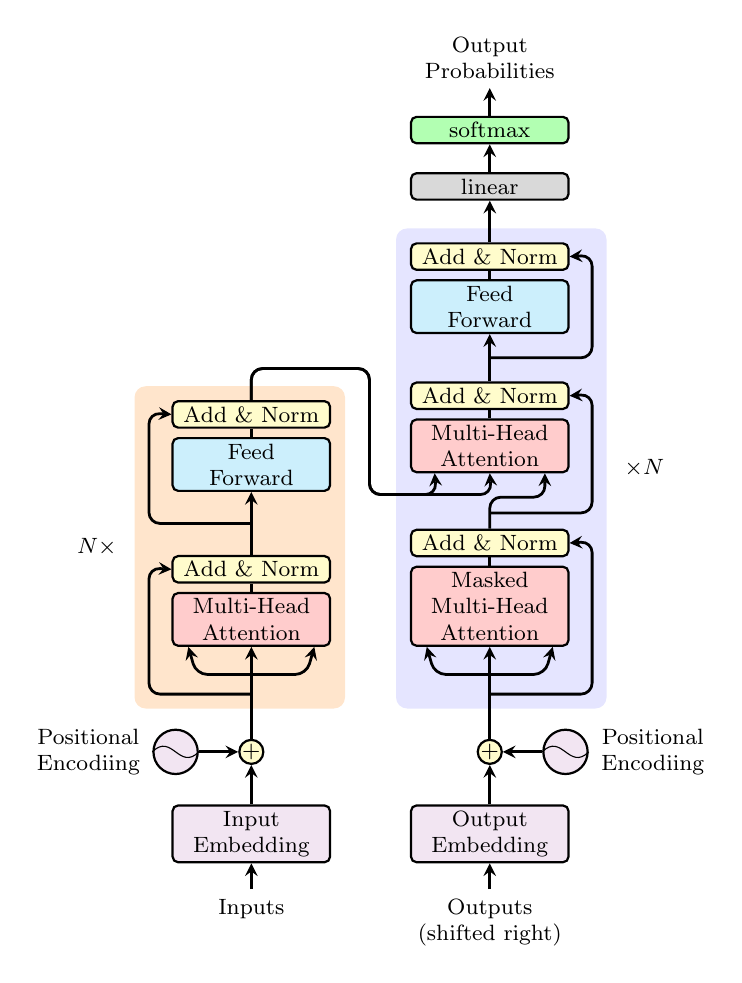
\begin{tikzpicture}
	\tikzstyle{input} = [draw,thick,inner sep=2pt,rounded corners=2pt,font=\footnotesize,fill=violet!10,,align=center,minimum width=2cm]
    \tikzstyle{multi-head} = [draw,thick,inner sep=2pt,rounded corners=2pt,font=\footnotesize,fill=red!20,align=center,minimum width=2cm]
    \tikzstyle{feed} = [draw,thick,inner sep=2pt,rounded corners=2pt,font=\footnotesize,fill=cyan!20,align=center,minimum width=2cm]
    \tikzstyle{add} = [draw,thick,inner sep=2pt,rounded corners=2pt,font=\footnotesize,fill=yellow!20,align=center,minimum width=2cm]
    \tikzstyle{pos-eb} = [circle,draw,thick,inner sep=0pt,fill=yellow!20,font=\footnotesize]
    \tikzstyle{curve-arrow} = [-stealth,line width=1pt,rounded corners]
    
    %left part
    \node [input] (src-eb) at (0,0){Input \\ Embedding};
    \node [anchor=south,pos-eb,minimum size=0.1em] (src-dc) at ([yshift=0.5cm]src-eb.north){+};
    \node [anchor=east,pos-eb,minimum size=1.6em,fill=violet!10] (src-pos) at ([xshift=-0.5cm]src-dc.west){};
    \node [anchor=south,multi-head] (en-multi) at ([yshift=2cm]src-eb.north){Multi-Head \\ Attention};
    \node [anchor=south,add] (en-add1) at ([yshift=0.3em]en-multi.north){Add \& Norm};
    \node [anchor=south,feed] (en-feed) at ([yshift=0.8cm]en-add1.north){Feed \\ Forward};
    \node [anchor=south,add] (en-add2) at ([yshift=0.3em]en-feed.north){Add \& Norm};

    %right part
    \node [anchor=west,input] (tgt-eb) at ([xshift=1cm]src-eb.east){Output \\ Embedding};
    \node [anchor=south,pos-eb,minimum size=0.1em] (tgt-dc) at ([yshift=0.5cm]tgt-eb.north){+};
    \node [anchor=west,pos-eb,minimum size=1.6em,fill=violet!10] (tgt-pos) at ([xshift=0.5cm]tgt-dc.east){~};
    \node [anchor=south,multi-head] (de-multi) at ([yshift=2cm]tgt-eb.north){Masked \\ Multi-Head \\ Attention};
    \node [anchor=south,add] (de-add1) at ([yshift=0.3em]de-multi.north){Add \& Norm};
    \node [anchor=south,multi-head] (en-de-multi) at ([yshift=2em]de-add1.north){Multi-Head \\ Attention};
    \node [anchor=south,add] (de-add2) at ([yshift=0.3em]en-de-multi.north){Add \& Norm};
    \node [anchor=south,feed] (de-feed) at ([yshift=0.6cm]de-add2.north){Feed \\ Forward};
    \node [anchor=south,add] (de-add3) at ([yshift=0.3em]de-feed.north){Add \& Norm};
    \node [anchor=south,add,fill=gray!30] (linear) at ([yshift=1.5em]de-add3.north){linear};
    \node [anchor=south,add,fill=green!30] (softmax) at ([yshift=1em]linear.north){softmax};

    %text outside
    \node [anchor=south,align=center,font=\footnotesize] (output-pro) at ([yshift=1em]softmax.north){Output \\ Probabilities};
    \node [anchor=north,align=center,font=\footnotesize] (tgt) at ([yshift=-2em]tgt-eb){Outputs \\ (shifted right)};
    \node [anchor=north,align=center,font=\footnotesize] (src) at ([yshift=-2em]src-eb){Inputs};
    \node [anchor=east,align=center,font=\footnotesize] (pos-eb1) at ([xshift=-0.1em]src-pos.west){Positional \\ Encodiing};
    \node [anchor=west,align=center,font=\footnotesize] (pos-eb2) at ([xshift=0.1em]tgt-pos.east){Positional \\ Encodiing};

    %left line
    \draw[-stealth,line width=1pt] (src.north) -- (src-eb.south);
    \draw[-stealth,line width=1pt] (src-eb.north) -- (src-dc.south);
    \draw[-stealth,line width=1pt] (src-pos.east) -- (src-dc.west);
    \draw[-stealth,line width=1pt] (src-dc.north) -- (en-multi.south);
    \draw[-,line width=1pt] (en-multi.north) -- (en-add1.south);
    \draw[-stealth,line width=1pt] (en-add1.north) -- (en-feed.south);
    \draw[-,line width=1pt] (en-feed.north) -- (en-add2.south);
    \draw[stealth-stealth,line width=1pt,rounded corners] ([xshift=-0.8cm]en-multi.south) -- ([xshift=-0.7cm,yshift=-0.35cm]en-multi.south) -- ([xshift=0.7cm,yshift=-0.35cm]en-multi.south) -- ([xshift=0.8cm]en-multi.south);
    \draw[curve-arrow] ([yshift=-0.6cm]en-multi.south) -- ([xshift=-1.3cm,yshift=-0.6cm]en-multi.south) -- ([xshift=-1.3cm,yshift=0.2cm]en-add1.south) -- (en-add1.west);
    \draw[curve-arrow] ([yshift=-0.4cm]en-feed.south) -- ([xshift=-1.3cm,yshift=-0.4cm]en-feed.south) -- ([xshift=-1.3cm,yshift=0.2cm]en-add2.south) -- (en-add2.west);

    %right line
    \draw[-stealth,line width=1pt] (tgt.north) -- (tgt-eb.south);
    \draw[-stealth,line width=1pt] (tgt-eb.north) -- (tgt-dc.south);
    \draw[-stealth,line width=1pt] (tgt-pos.west) -- (tgt-dc.east);
    \draw[-stealth,line width=1pt] (tgt-dc.north) -- (de-multi.south);
    \draw[-,line width=1pt] (de-multi.north) -- (de-add1.south);
    \draw[-,line width=1pt] (en-de-multi.north) -- (de-add2.south);
    \draw[-stealth,line width=1pt] (de-add2.north) -- (de-feed.south);
    \draw[-,line width=1pt] (de-feed.north) -- (de-add3.south);
    \draw[-stealth,line width=1pt] (de-add3.north) -- (linear.south);
    \draw[-stealth,line width=1pt] (softmax.north) -- (output-pro.south);
    \draw[-stealth,line width=1pt] (linear.north) -- (softmax.south);
    \draw[stealth-stealth,line width=1pt,rounded corners] ([xshift=-0.8cm]de-multi.south) -- ([xshift=-0.7cm,yshift=-0.35cm]de-multi.south) -- ([xshift=0.7cm,yshift=-0.35cm]de-multi.south) -- ([xshift=0.8cm]de-multi.south);
    \draw[curve-arrow] ([yshift=-0.6cm]de-multi.south) -- ([xshift=1.3cm,yshift=-0.6cm]de-multi.south) -- ([xshift=1.3cm,yshift=0.2cm]de-add1.south) -- (de-add1.east);
    \draw[curve-arrow](en-add2.north) -- ([yshift=0.4cm]en-add2.north) -- ([yshift=0.4cm,xshift=1.5cm]en-add2.north) -- ([yshift=-1.2cm,xshift=1.5cm]en-add2.north) -- ([yshift=-1.2cm,xshift=2.35cm]en-add2.north) -- ([xshift=-0.7cm]en-de-multi.south);
    \draw[curve-arrow](en-add2.north) -- ([yshift=0.4cm]en-add2.north) -- ([yshift=0.4cm,xshift=1.5cm]en-add2.north) -- ([yshift=-1.2cm,xshift=1.5cm]en-add2.north) -- ([yshift=-1.2cm,xshift=3.05cm]en-add2.north) -- (en-de-multi.south);
    \draw[curve-arrow](de-add1.north) -- ([yshift=0.4cm]de-add1.north) -- ([yshift=0.4cm,xshift=0.7cm]de-add1.north) -- ([xshift=0.7cm]en-de-multi.south);
    \draw[curve-arrow]([yshift=0.2cm]de-add1.north) -- ([yshift=0.2cm,xshift=1.3cm]de-add1.north) -- ([yshift=0.2cm,xshift=1.3cm]de-add2.south) -- (de-add2.east);
    \draw[curve-arrow] ([yshift=-0.3cm]de-feed.south) -- ([xshift=1.3cm,yshift=-0.3cm]de-feed.south) -- ([xshift=1.3cm,yshift=0.2cm]de-add3.south) -- (de-add3.east);
    
    %position embeding
    \draw[-] (src-pos.west) .. controls +(north east:1em) and +(south west:1em)..(src-pos.east);
    \draw[-] (tgt-pos.west) .. controls +(north east:1em) and +(south west:1em)..(tgt-pos.east);
    
    %padding
    \node [minimum size=1cm] (k1) at ([xshift=-0.8cm,yshift=-0.1cm]en-multi.south){};
    \node [minimum size=1cm] (k2) at ([xshift=0.8cm,yshift=-0.1cm]de-multi.south){};
    
    %background
    \begin{pgfonlayer}{background}
        \node [rectangle,inner sep=0.5em,fill=orange!20,rounded corners=4pt] [fit = (en-multi) (en-add1) (en-feed) (en-add2) (k1)] (box0) {};
        \node [rectangle,inner sep=0.5em,fill=blue!10,rounded corners=4pt] [fit = (de-multi) (de-add1) (en-de-multi) (de-add2) (de-feed) (de-add3) (k2)] (box1) {};
        
    \node [anchor=west,align=center,font=\footnotesize](de_n) at ([xshift=0.1cm]box1.east){$\times N$};
    \node [anchor=east,align=center,font=\footnotesize](en_n) at ([xshift=-0.1cm]box0.west){$N \times$};
    \end{pgfonlayer}
	\end{tikzpicture}
    \end{spacing}
\end{document} 